%!TEX root = ../main.tex

%=======================================================================  hyperbola
\section{Hyperbola}
\label{sec:hyperbola}

	The \emphindexdef{hyperbola} is another fundamental shape of nature.
	

	\subsection{The conic sections}

		There is a deep connection between the geometric shapes of the circle,
		the ellipse, the parabola, and the hyperbola.
		These seemingly different shapes can be obtained, geometrically speaking,
		from a single object: the cone.															\index{cone}
		We can obtain the four curves by slicing the cone at different angles,
		as illustrated in Figure~\ref{fig:conic_sections_four-shapes}.

		\begin{figure}[htb]
			\centering
			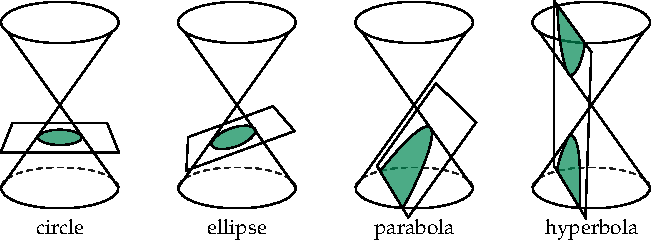
\includegraphics[width=0.8\textwidth]{figures/math/conic_sections_four-shapes.pdf}
			\vspace{-2mm}
			\caption{	Taking slices through a cone at different angles produces different geometric shapes:
					a circle, an ellipse, a parabola, or a hyperbola.}
			\label{fig:conic_sections_four-shapes}
		\end{figure}
	

	\subsection{Conic sections in polar coordinates}

		All four conic sections can be described by the same function in polar coordinates:					\index{polar coordinates}
		\[
		  r(\theta) = \frac{q(1+\varepsilon)}{1 + \varepsilon\cos(\theta)}\,,
		\]
		where $q$ is the curve's closest distance to a focal point
		and $\varepsilon$ is the curve's eccentricity.												\index{eccentricity}
		For a circle, $q=R$ (the radius) and the eccentricity parameter is $\varepsilon=0$.
		For an ellipse, $q=a(1-\varepsilon)$ and the eccentricity parameter varies between $0$ and $1$ ($0\leq \varepsilon < 1$).
		Note we include the case $\varepsilon=0$ since a circle is a special case of an ellipse.
		For a parabola, $q=f$ (the focal length) and the eccentricity is $\varepsilon=1$.
		For a hyperbola, $q = a(\varepsilon-1)$ and the eccentricity is $\varepsilon>1$.

		We can use the eccentricity parameter $\varepsilon$ to classify all four curves.
		Depending on the value of $\varepsilon$,
		the equation $r(\theta)$ defines either a circle, an ellipse, a parabola, or a hyperbola.	\index{circle}\index{ellipse}\index{hyperbola}\index{parabola}
		Table~\ref{table:conics} summarizes all our observations regarding conic sections.


		\begin{table}[htb]
		{ \small

		\centering 
		\begin{longtable}{@{}lllll@{}} 
		\toprule
		Conic section 	\! 	&  Equation  	\!\!					
		& Polar function	
		&	Eccentricity \!\!\!\!\!\!\!\!\!\!\!\!				\\
		\midrule
		Circle				& $x^2+y^2=R^2$ \; 					& $r(\theta)=R$			& $\varepsilon = 0$								\\[1mm]
		Ellipse				& $\frac{x^2}{a^2}+\frac{y^2}{b^2}=1$	& $r(\theta)=\frac{a(1-\varepsilon^2)}{1 + \varepsilon\cos(\theta)}$ &	$\varepsilon\!=\!\sqrt{1\!-\!\frac{b^2}{a^2}}\,, \; 0\!\leq\!\varepsilon\!<\!1$\!\!	\\[2mm]
		Parabola				& $y^2=4fx$						& $r(\theta)=\frac{2f}{1 + \cos(\theta)}$ &	$\varepsilon=1$			 						\\[1mm]
		Hyperbola			& $\frac{x^2}{a^2}-\frac{y^2}{b^2}=1$	& $r(\theta)=\frac{a(\varepsilon^2-1)}{1 + \varepsilon\cos(\theta)}$ &	$\varepsilon\!=\!\sqrt{1\!+\!\frac{b^2}{a^2}}\,, \; 1\!<\!\varepsilon\!<\!\infty$ \\[1mm]
		\bottomrule
		\end{longtable}

		}
		\vspace{4mm}
		\caption{The four conic sections and their eccentricity parameters. }
		\label{table:conics}
		\end{table}


		The motion of the planets is explained by Newton's law of gravitation.
		The gravitational interaction between two bodies always leads one of the two bodies to follow a trajectory described by one of the conic sections
		for which the other body is the focal point.
